% \documentclass[handout]{beamer}
\documentclass{beamer}

\mode<presentation>
{
  \usetheme{default}
  \usefonttheme[onlymath]{serif}
  % \usetheme{Singapore}
  % \usetheme{Warsaw}
  % \usetheme{Malmoe}
  % \useinnertheme{circles}
  % \useoutertheme{infolines}
  % \useinnertheme{rounded}

  \setbeamercovered{transparent=100}
}

\usepackage[english]{babel}
\usepackage[latin1]{inputenc}
\usepackage{alltt,listings,multirow,ulem,siunitx}
\usepackage[absolute,overlay]{textpos}
\TPGrid{1}{1}
\usepackage{pdfpages}
\usepackage{multimedia}
\usepackage{multicol}
\newcommand\hmmax{0}
\newcommand\bmmax{0}
\usepackage{bm}
\usepackage{comment}

% font definitions, try \usepackage{ae} instead of the following
% three lines if you don't like this look
\usepackage{mathptmx}
\usepackage[scaled=.90]{helvet}
% \usepackage{courier}
\usepackage[T1]{fontenc}
\usepackage{tikz}
\usetikzlibrary{decorations.pathreplacing}
\usetikzlibrary{shadows,arrows,shapes.misc,shapes.arrows,shapes.multipart,arrows,decorations.pathmorphing,backgrounds,positioning,fit,petri,calc,shadows,chains,matrix,mindmap}
%\usetikzlibrary[shapes,shapes.arrows,arrows,shapes.misc,fit,positioning,trees,mindmap,backgrounds]



% \usepackage{pgfpages}
% \pgfpagesuselayout{4 on 1}[a4paper,landscape,border shrink=5mm]

\usepackage{JedMacros}

\newcommand{\timeR}{t_{\mathrm{R}}}
\newcommand{\timeW}{t_{\mathrm{W}}}
\newcommand{\mglevel}{\ensuremath{\ell}}
\newcommand{\mglevelcp}{\ensuremath{\mglevel_{\mathrm{cp}}}}
\newcommand{\mglevelcoarse}{\ensuremath{\mglevel_{\mathrm{coarse}}}}
\newcommand{\mglevelfine}{\ensuremath{\mglevel_{\mathrm{fine}}}}

%solution and residual
\newcommand{\vx}{\ensuremath{x}}
\newcommand{\vc}{\ensuremath{\hat{x}}}
\newcommand{\vr}{\ensuremath{r}}
\newcommand{\vb}{\ensuremath{b}}

%operators
\newcommand{\vA}{\ensuremath{A}}
\newcommand{\vP}{\ensuremath{I_H^h}}
\newcommand{\vS}{\ensuremath{S}}
\newcommand{\vR}{\ensuremath{I_h^H}}
\newcommand{\vI}{\ensuremath{\hat I_h^H}}
\newcommand{\vV}{\ensuremath{\mathbf{V}}}
\newcommand{\vF}{\ensuremath{F}}
\newcommand{\vtau}{\ensuremath{\mathbf{\tau}}}


\title{Discretization, Solvers, and Statistics in Computational Geodynamics}
\subtitle{{\normalsize \url{http://59A2.org/files/20130423-EarthCube.pdf}}}
\author{{\bf Jed Brown}}

% - Use the \inst command only if there are several affiliations.
% - Keep it simple, no one is interested in your street address.
\institute
{
  {Mathematics and Computer Science Division, Argonne National Laboratory}
}

\date{EarthCube, Boulder, CO, 2013-04-23}

% This is only inserted into the PDF information catalog. Can be left
% out.
\subject{Talks}


% If you have a file called "university-logo-filename.xxx", where xxx
% is a graphic format that can be processed by latex or pdflatex,
% resp., then you can add a logo as follows:

% \pgfdeclareimage[height=0.5cm]{university-logo}{university-logo-filename}
% \logo{\pgfuseimage{university-logo}}



% Delete this, if you do not want the table of contents to pop up at
% the beginning of each subsection:
% \AtBeginSubsection[]
% {
% \begin{frame}<beamer>
%   \frametitle{Outline}
%   \tableofcontents[currentsection,currentsubsection]
% \end{frame}
% }

\AtBeginSection[]
{
  \begin{frame}<beamer>
    \frametitle{Outline}
    \tableofcontents[currentsection]
  \end{frame}
}

% If you wish to uncover everything in a step-wise fashion, uncomment
% the following command:

% \beamerdefaultoverlayspecification{<+->}

\begin{document}
\lstset{language=C}
\normalem

\begin{frame}
  \titlepage
\end{frame}

\begin{frame}{Challenges}
  \begin{itemize}
  \item Discretization
    \begin{itemize}
    \item high accuracy
    \item heterogeneity and homogenization
    \item tracers for material properties
    \end{itemize}
  \item Solvers
    \begin{itemize}
    \item stiff transient systems
    \item elliptic problems
    \item globalization for nonlinear problems
    \end{itemize}
  \item Statistics
    \begin{itemize}
    \item Seismic tomography
    \item Data assimilation and validation
    \item Experimental design
    \end{itemize}
  \item Reusability and reproducibility
    \begin{itemize}
    \item Libraries\footnote{Disclaimer: I am a developer of PETSc.}
    \item Common formats
    \item Shared simulation software
    \end{itemize}
  \end{itemize}
\end{frame}

\begin{frame}
  \begin{center}
    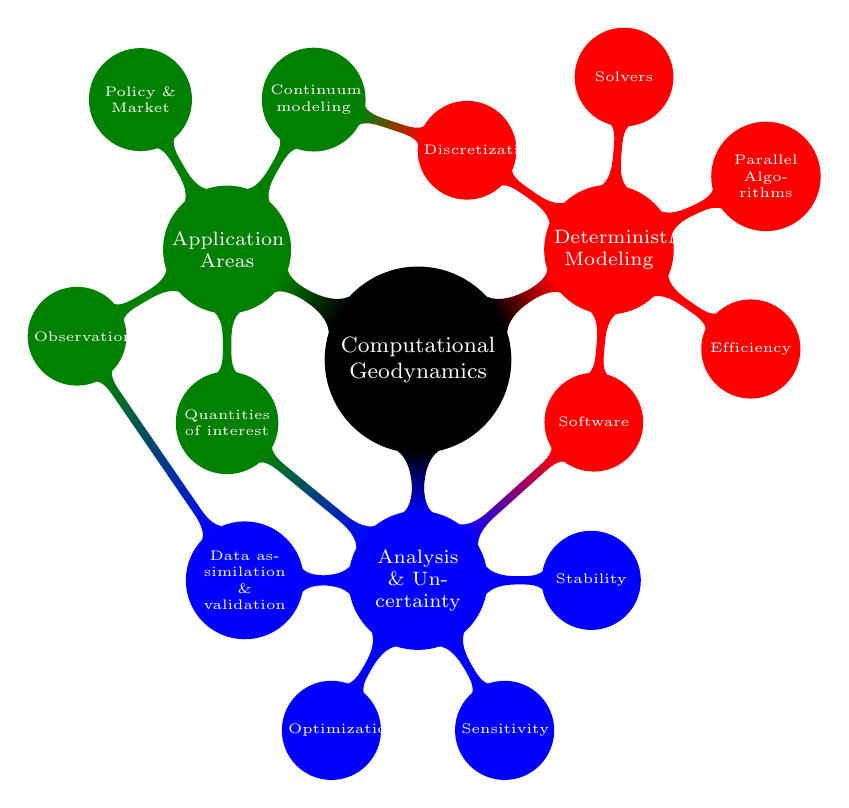
\begin{tikzpicture}
      [small mindmap,concept color=black,text=white,
      %level 1 concept/.append style={level distance=120,sibling angle=30},
      extra concept/.append style={color=blue!50,text=black}]

      \node [concept] {Computational Geodynamics}
      child [concept color=green!50!black,grow=150] {
        node [concept] {Application \\ Areas}[counterclockwise from=60]
        child {node [concept] (cont) {Continuum modeling}}
        child {node [concept] (policy) {Policy \& Market}}
        child[grow=-150] {node [concept] (obs) {Observation}}
        child[grow=-90] {node [concept] (qoi) {Quantities of interest}}
      }
      child [concept color=red,text=white,grow=30] {
        node [concept] {Deterministic Modeling}[clockwise from=145,sibling angle=25]
        child {node [concept] (disc) {Discretization}}
        child {node [concept] (solver) {Solvers}}
        child {node [concept] (alg) {Parallel Algorithms}}
        child {node [concept] (eff) {Efficiency}}
        child {node [concept] (software) {Software}}
      }
      child [concept color=blue,text=white,grow=-90] {
        node[concept] (analysis) {Analysis \& Uncertainty}[clockwise from=0]
        child {node [concept] (stab) {Stability}}
        child {node [concept] (sens) {Sensitivity}}
        child {node [concept] (opt) {Optimization}}
        child {node [concept] (assim) {Data assimilation \\ \& validation}}
      }
      ;
      \begin{pgfonlayer}{background}
        \path (analysis) to[circle connection bar switch color=from (blue) to (red)] (software);
        \path (cont) to[circle connection bar switch color=from (green!50!black) to (red)] (disc);
        \path (qoi) to[circle connection bar switch color=from (green!50!black) to (blue)] (analysis);
        \path (obs) to[circle connection bar switch color=from (green!50!black) to (blue)] (assim);
      \end{pgfonlayer}
    \end{tikzpicture}
  \end{center}
\end{frame}

\begin{frame}{SPECFEM3D: Seismic wave propagation and tomography}
  \begin{itemize}
  \item Spectral element methods: accurate, local, smooth solutions
  \item Linear materials
  \item Adjoint-based tomography
  \item \url{http://geodynamics.org/cig/software/specfem3d}
  \end{itemize}
  \includegraphics[width=\textwidth]{figures/TapeCookInlet.png} \\
  {[c/o Carl Tape, UAF]}
\end{frame}

\begin{frame}{PyLith: Short-term Lithosphere}
  \begin{textblock}{0.3}[1,0](0.99,0.1)
    \includegraphics[width=\textwidth]{figures/PyLithCover.png}
  \end{textblock}
  \vspace{3em}
  \begin{itemize}
  \item Unstructured finite element methods
  \item Faults meshed-in (CUBIT, LaGriT)
  \item Cohesive cells and Lagrange multipliers
  \item Nonlinear materials and non-smooth behavior
  \item Extensible material models and boundary conditions
  \item Long time scales requires implicit solvers: fieldsplit and multigrid
  \item Libraries: PETSc (mesh and solvers), spatialdata (proj), numpy, FIAT (elements), HDF5
  \item \url{http://geodynamics.org/cig/software/pylith}
  \end{itemize}
\end{frame}

% Seismic, short-term lithosphere, long-term lithosphere, mantle, geodynamo

\begin{frame}{Stokes problems are ubiquitous in long-term geodynamics}
  \begin{gather*}
    \nabla\cdot (-\eta D \bm u + p\bm 1) = \rho \bm g \\
    \nabla\cdot \bm u = c
  \end{gather*}
  \vspace{-2ex}
  \begin{itemize}
  \item $D\bm u = \frac 1 2 \big[ \nabla \bm u + (\nabla \bm u)^T \big]$, rheology $\eta(D\bm u,\dotsc)$
  \item Mantle, lithosphere, magma
  \item Coupled to other processes
    \begin{itemize}
    \item Thermodynamics
    \item Multi-material transport, chemistry
    \item Plasticity/brittle failure: difficult non-smooth
    \item Elasticity: typical Maxwell time of 1000 years
    \end{itemize}
  \item Discontinuous coefficients: $10^{10}$ jumps
  \item Material properties defined using markers
  \item Discretization is difficult
    \begin{itemize}
    \item Trade-offs between accuracy, robustness, and efficiency
    \item What can go wrong?  Next sequence from Dave May (ETHZ)
    \end{itemize}
  \end{itemize}
\end{frame}

{
\setbeamercolor{background canvas}{bg=}
\includepdf[pages=1-7]{slides/Stokes/DaveMayQ1Q1.pdf}
}

\begin{frame}{Material transport using markers}
  \includegraphics[width=\textwidth]{figures/MayMarkersHomogenization.png} \\
  {\scriptsize [c/o Dave May, ETHZ]}
\end{frame}

\begin{frame}{Algorithms keep pace with computing}
  \begin{itemize}
  \item Consider an elliptic PDE on an $n\times n \times n$ grid
  \item Banded Gaussian Elimination: $\bigO(n^7)$
  \item Full Multigrid: $\bigO(n^3)$
  \item Optimal algorithms become more critical as we solve larger problems
  \end{itemize}
  \includegraphics[width=0.9\textwidth]{figures/KeyesAlgorithmsKeepPace.png} \\
  {[c/o David Keyes, KAUST]}
\end{frame}

\begin{frame}{The Great Solver Schism: Monolithic or Split?}
  \begin{columns}
    \begin{column}{0.5\textwidth}
      \begin{block}{Monolithic}
        \begin{itemize}
        \item Direct solvers
        \item Coupled Schwarz
        \item Coupled Neumann-Neumann \\
          (need unassembled matrices)
        \item Coupled multigrid
        \item[X] Need to understand local spectral and compatibility properties of the coupled system
        \end{itemize}
      \end{block}
    \end{column}
    \begin{column}{0.5\textwidth}
      \begin{block}{Split}
        \begin{itemize}
        \item Physics-split Schwarz \\
          (based on relaxation)
        \item Physics-split Schur \\
          (based on factorization)
          \begin{itemize}
          \item  approximate commutators \\
            SIMPLE, PCD, LSC
          \item segregated smoothers
          \item Augmented Lagrangian
          \item ``parabolization'' for stiff waves
          \end{itemize}
        \item[X] Need to understand global coupling strengths
        \end{itemize}
      \end{block}
    \end{column}
  \end{columns}
  \begin{itemize}
  \item Preferred data structures depend on which method is used.
  \item Interplay with geometric multigrid.
  \end{itemize}
\end{frame}

\begin{frame}{Splitting for Multiphysics}
  \begin{equation*}
    \begin{bmatrix}
      A & B \\ C & D
    \end{bmatrix}
    \begin{bmatrix}
      x \\ y
    \end{bmatrix}
    =
    \begin{bmatrix}
      f \\ g
    \end{bmatrix}
  \end{equation*}
  \begin{itemize}\item Relaxation:
    \code{-pc\_fieldsplit\_type [additive,multiplicative,symmetric\_multiplicative]}
    \begin{equation*}
      \begin{bmatrix}
        A & \\  & D
      \end{bmatrix}^{-1} \qquad 
      \begin{bmatrix}
        A & \\ C & D
      \end{bmatrix}^{-1} \qquad
      \begin{bmatrix}
        A & \\  & \bm 1
      \end{bmatrix}^{-1}
      \left(
        \bm 1 -
        \begin{bmatrix}
          A & B \\ & \bm 1
        \end{bmatrix}
        \begin{bmatrix}
          A & \\ C & D
        \end{bmatrix}^{-1}
      \right)
    \end{equation*}
    \begin{itemize}
    \item Gauss-Seidel inspired, works when fields are loosely coupled
    \end{itemize}
  \item Factorization: \code{-pc\_fieldsplit\_type schur}
    \begin{align*}
      \begin{bmatrix}
        A & B \\ & S
      \end{bmatrix}^{-1}
      \begin{bmatrix}
        1 & \\ CA^{-1} & 1
      \end{bmatrix}^{-1}, \qquad
      S = D - C A^{-1} B
    \end{align*}
    \begin{itemize}
    \item robust (exact factorization), can often drop lower block
    \item how to precondition $S$ which is usually dense?
      \begin{itemize}
      \item interpret as differential operators, use approximate commutators
      \end{itemize}
    \end{itemize}
  \end{itemize}
\end{frame}


\begin{frame}[fragile]{Multigrid Preliminaries}
  \begin{figure}
    \centering
    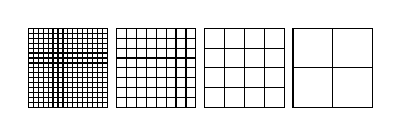
\begin{tikzpicture}
      [>=stealth,
      every node/.style={inner sep=2pt},
      restrict/.style={thick},
      prolong/.style={thick},
      mglevel/.style={rounded rectangle,draw=blue!50!black,fill=blue!20,thick,minimum size=4mm},
      ]
      \begin{scope}\scriptsize
        \newcommand\mgdx{4.0em}
        \newcommand\mgdy{4.0em}
        \newcommand\mgl[1]{(pow(2,#1+1))}
        \newcommand\mgloc[4]{(#1 + #4*\mgdx*#3,#2 + \mgdy*#3)}

        \newcommand\mghx{0.9*\mgdx}
        \newcommand\mghy{0.9*\mgdy}

        \draw[shift=\mgloc{0*\mgdx}{0}{0}{0},
        xstep=\mghy/\mgl{3},
        ystep=\mghy/\mgl{3}]
        (-0.5*\mghy,-0.5*\mghy) grid (0.5*\mghy,0.5*\mghy);

        \draw[shift=\mgloc{1*\mgdx}{0}{0}{0},
        xstep=\mghy/\mgl{2},
        ystep=\mghy/\mgl{2}]
        (-0.5*\mghy,-0.5*\mghy) grid (0.5*\mghy,0.5*\mghy);

        \draw[shift=\mgloc{2*\mgdx}{0}{0}{0},
        xstep=\mghy/\mgl{1},
        ystep=\mghy/\mgl{1}]
        (-0.5*\mghy,-0.5*\mghy) grid (0.5*\mghy,0.5*\mghy);


        \draw[shift=\mgloc{3*\mgdx}{0}{0}{0},
        xstep=\mghy/\mgl{0},
        ystep=\mghy/\mgl{0}]
        (-0.5*\mghy,-0.5*\mghy) grid (0.5*\mghy,0.5*\mghy);
      \end{scope}
    \end{tikzpicture}
    \label{fig:levels}
  \end{figure}
  \textbf{Multigrid} is an $O(n)$ method for solving algebraic problems by defining a hierarchy of scale.
  A multigrid method is constructed from:
  \begin{enumerate}
  \item a series of discretizations
    \begin{itemize}
    \item coarser approximations of the original problem
    \item constructed algebraically or geometrically
    \end{itemize}
  \item intergrid transfer operators
    \begin{itemize}
    \item residual restriction $I_h^H$ (fine to coarse)
    \item state restriction $\hat I_h^H$ (fine to coarse)
    \item partial state interpolation $I_H^h$ (coarse to fine, `prolongation')
    \item state reconstruction $\mathbb{I}_H^h$ (coarse to fine)
    \end{itemize}
  \item Smoothers ($S$)
    \begin{itemize}
    \item correct the high frequency error components
    \item Richardson, Jacobi, Gauss-Seidel, etc.
    \item Gauss-Seidel-Newton or optimization methods
    \end{itemize}
  \end{enumerate}
\end{frame}

\begin{frame}[fragile]
  \frametitle{Linear Multigrid}
  \begin{itemize}
    \item \textbf{Multigrid} methods use coarse correction for long-range influence
  \end{itemize}
  \begin{figure}
  \centering
  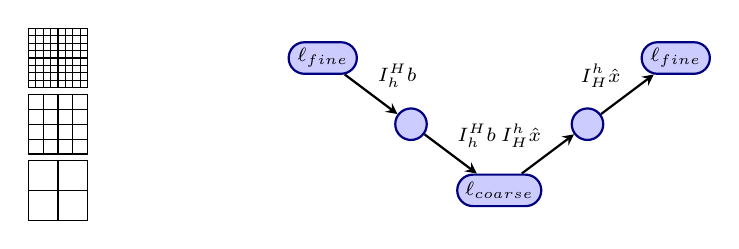
\begin{tikzpicture}
    [>=stealth,
    every node/.style={inner sep=2pt},
    restrict/.style={thick},
    prolong/.style={thick},
    mglevel/.style={rounded rectangle,draw=blue!50!black,fill=blue!20,thick,minimum size=4mm},
    ]
    \begin{scope}\scriptsize
      \newcommand\mgdx{4.0em}
      \newcommand\mgdy{3.0em}
      \newcommand\mgl[1]{(pow(2,#1+1))}
      \newcommand\mgloc[4]{(#1 + #4*\mgdx*#3,#2 + \mgdy*#3)}
      \node[mglevel] (down0) at \mgloc{0}{0}{2}{-1} {\mglevel$_{fine}$};
      \node[mglevel] (down1) at \mgloc{0}{0}{1}{-1} {};
      \node[mglevel] (coarse) at \mgloc{0}{0}{0}{-1} {\mglevel$_{coarse}$};

      \node[mglevel] (up1) at \mgloc{0}{0}{1}{1} {};
      \node[mglevel] (up0) at \mgloc{0}{0}{2}{1} {\mglevel$_{fine}$};

      \path[->,restrict] (down0) edge node [above right] {$\vR\vb$} (down1)
                         (down1) edge node [above right] {$\vR\vb$} (coarse);

      \path[->,prolong] (coarse) edge node [above left] {$\vP\vc$} (up1)
                         (up1) edge node [above left] {$\vP\vc$} (up0);

      %grids
      \newcommand\mghx{0.9*\mgdx}
      \newcommand\mghy{0.9*\mgdy}

      \draw[shift=\mgloc{-5*\mgdx}{0}{2}{0},
      xstep=\mghy/\mgl{2},
      ystep=\mghy/\mgl{2}]
      (-0.5*\mghy,-0.5*\mghy) grid (0.5*\mghy,0.5*\mghy);

      \draw[shift=\mgloc{-5*\mgdx}{0}{1}{0},
      xstep=\mghy/\mgl{1},
      ystep=\mghy/\mgl{1}]
      (-0.5*\mghy,-0.5*\mghy) grid (0.5*\mghy,0.5*\mghy);

      \draw[shift=\mgloc{-5*\mgdx}{0}{0}{0},
      xstep=\mghy/\mgl{0},
      ystep=\mghy/\mgl{0}]
      (-0.5*\mghy,-0.5*\mghy) grid (0.5*\mghy,0.5*\mghy);

  \end{scope}
\end{tikzpicture}
\label{fig:MG}
\end{figure}
Algorithm $MG(\vA,\vb)$ for the solution of $\vA\vx = \vb$:
\begin{align*}
  &\vx = \vS^m(\vx,\vb)             & \text{pre-smooth}\\
  &\vb^{H} = \vR(\vr - \vA\vx)       & \text{restrict residual}\\
  &\vc^{H} = MG(\vR\vA\vP,\vb^{H})   & \text{recurse}\\
  &\vx = \vx + \vP\vc^{H}            & \text{prolong correction}\\
  &\vx = \vx + \vS^n(\vx,\vb)       & \text{post-smooth}\\
\end{align*}
\end{frame}

\begin{frame}{Status quo for implicit solves in lithosphere dynamics}
  \begin{itemize}
  \item global linearization using Newton or Picard
  \item assembly of a sparse matrix
  \item ``block'' factorization preconditioner, approximate Schur complement
  \item algebraic or geometric multigrid on positive-definite systems
  \end{itemize}
  \begin{block}{Why is this bad?}
    \vspace{-1em}
    \begin{itemize}
    \item nonlinearities (e.g., plastic yield) are mostly local
      \begin{itemize}
      \item feed back through nearly linear large scales
      \item frequent visits to fine-scales even in nearly-linear regions
      \item no way to locally update coarse grid operator
      \item Newton linearization introduces anisotropy
      \end{itemize}
    \item assembled sparse matrices are terrible for performance on modern hardware
      \begin{itemize}
      \item memory bandwidth is very expensive compared to flops
      \item fine-scale assembly costs a lot of memory
      \item assembled matrices are good for algorithmic experimentation
      \end{itemize}
    \item block preconditioners require more parallel communication
    \end{itemize}
  \end{block}
\end{frame}

\begin{frame}{Reproducibility}
  \begin{itemize}
  \item Geometry, Boundary, and Initial conditions
  \item Model configuration has poor reproducibility and automation
    \begin{itemize}
    \item CAD software to create geometry
    \item Interactive meshing (CUBIT)
    \item Observational metadata
      \begin{itemize}
      \item lack of uncertainties, correlation
      \item diverse data sources, hard to quantify value
      \end{itemize}
    \item Interactive postprocessing
    \end{itemize}
  \item Model execution \emph{can} be reproducible
    \begin{itemize}
    \item Exact versions in SCM (Git, Subversion)
    \item Compilers, dependencies, configure- and run-time options
    \item Postprocessing scripts
    \end{itemize}
  \end{itemize}
\end{frame}

\begin{frame}{Data assimilation and experimental design}
  \begin{itemize}
  \item Impact of geodynamics
    \begin{itemize}
    \item Fundamental science questions
    \item Hazards, safety, construction
    \item Industry: minerals, petroleum
    \end{itemize}
  \item Analysis tools more mature for faster processes
    \begin{itemize}
    \item Short time scales and ``single-physics'' processes
    \item Seismic tomography serves both science and industry
    \end{itemize}
  \item More ad-hoc for longer term processes
    \begin{itemize}
    \item More diverse data sources
    \item Extremely indirect observations
    \item Little meaning inferrable using single-physics models
    \item Uncertainty propagation is under-developed
    \item Non-smooth processes are troublesome for adjoints
    \end{itemize}
  \item What measurements provide the most information?
  \end{itemize}  
\end{frame}
% Attempting to scale people.  Good solver algorithms have more interplay with spatial discretization, but poorer
% modularity.

% Visualization/analysis cannot be based on writing complete model state to disk.

\begin{frame}{Looking forward}
  \begin{itemize}
  \item Is it good for everyone to write their own models?
    \begin{itemize}
    \item Diversity is good for improving models
    \item Creating a complete model from scratch is a lot of mundane work
    \item Common interfaces allow users to compare multiple models
    \item Libraries are a maintainable way to provide long-term reuse
    \item Few models start out as libraries, some become libraries
    \item Coupling necessary to understand long-term processes
    \end{itemize}
  \item Scaling people
    \begin{itemize}
    \item ``Experts in everything'' are valuable, but hard to find
    \item The best algorithms remove comfortable abstractions like sparse matrices
    \item Many open research topics: difficult to establish interfaces
    \end{itemize}
  \item Postprocessing
    \begin{itemize}
    \item Status quo is to write entire state to disk --- not sustainable
    \item Think like an engineer: ask precise questions --- good for reproducibility
    \end{itemize}
  \end{itemize}
\end{frame}

\end{document}
